\documentclass[a4paper, 10pt]{article}
\hyphenpenalty=8000
\textwidth=125mm
\textheight=185mm

\usepackage{algorithm}
\usepackage{algpseudocode} % Per il linguaggio di pseudo-codice

\usepackage{amsmath}  % Per migliorare la gestione delle formule
\usepackage{amssymb}  % Per simboli aggiuntivi come \mathbb

\usepackage{float}

\usepackage{graphicx}
\usepackage{subcaption}

%this package is flexible for image insertion
%
\usepackage{alltt}
%this package is suitable for the description of algorithms and computer programs
%
\usepackage{amsmath}
%this package draws mathematical symbols smoothly
%
\usepackage[hidelinks, pdftex]{hyperref}
%this package produces hypertext links in the document

\pagenumbering{arabic}
\setcounter{page}{1}
\renewcommand{\thefootnote}{\fnsymbol{footnote}}
\floatname{algorithm}{Procedura}


\begin{document}

\begin{center}

\LARGE
\textbf{Weighted Feedback Vertex Set Problem}\\[6pt]

\text{Progetto Intelligenza Artificiale} \\
\text{A.A. 2024/2025}\\

{\fontsize{15pt}{0pt}\selectfont Denise Cilia}\\
{\fontsize{15pt}{0pt}\selectfont 1000066023}\\

\end{center}

\bigskip
\bigskip



\section{Introduzione al problema}\label{s:1}
Uno dei primi problemi NP-completi di ottimizzazione presente nella teoria dei grafi è il \textit{Feedback Vertex Set Problem}. La sua risoluzione trova varie utili applicazioni nello studio delle situazioni di \textit{deadlock} presenti nei sistemi operativi e nella computazione parallela e in ulteriori scenari complessi. \\
Formalmente, dato un grafo non orientato $G = (V, E)$, il \textit{Feedback Vertex Set} (abbreviato in $\mathit{FVS}$) di G è un sottoinsieme $F\subseteq V$ di vertici la cui rimozione, compresa di archi, fornisce come risultato un grafo aciclico tale che $G(V\backslash S, E \backslash S)$ sia un grafo aciclico. In maniera equivalente, ciascun ciclo presente in $G$ contiene almeno un vertice in $F$. Sia inoltre $w: V \to \mathbb{R}^+$ la funzione peso che associa un valore positivo a ciascun vertice $v \in V$ in $G$, allora il peso dell'insieme \textit{Feedback Vertex Set} $F\subseteq V$ è dato dalla somma di tutti i pesi dei vertici. Per definizione:

\begin{center}
$\sum_{v\in F} w(v)$.
\label{eq:fvs_minimum_weight}
\end{center}

\noindent
Per lo studio in questione, verrà analizzato il \textit{Weighted Feedback Vertex Problem} ($\mathit{WFVP}$) su un grafo pesato $G$ che consiste nel minimizzare la somma dei pesi dei vertici contenuti in $F$ tale che:

\begin{center}
$min \sum_{v \in F} w(v)$.
\end{center}

\begin{figure}[H]
    \centering
    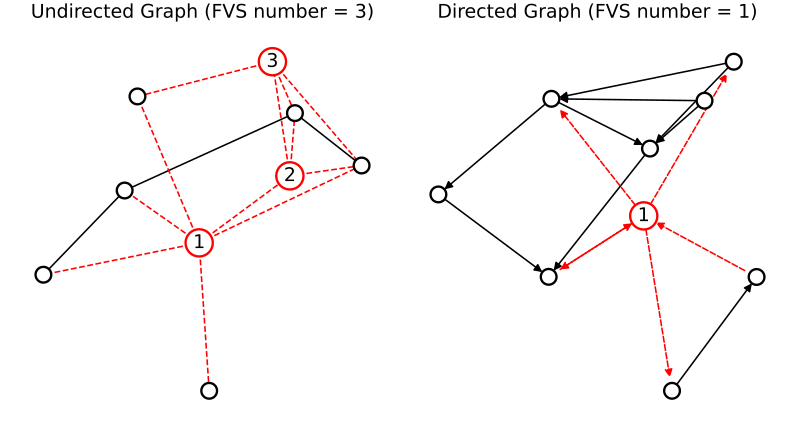
\includegraphics[width=0.50\textwidth]{./img/800px-Feedback_vertex_set.png}
    \caption{FVS Example}
    \label{fig:fvs_example}
\end{figure}

\noindent
Per poter analizzare questa tipologia di problema, lo studio propone l'applicazione dell'algoritmo \textit{Tabu Search} ($TS$) con lo scopo di risolvere in tempo lineare il problema e di avvicinarsi quanto più possibile ai migliori valori calcolati sinora. Si cercheranno i parametri adatti insieme alle migliori strategie per un'efficace esecuzione dell'algorit\-mo.


\section{Tabu Search}\label{s:2}
\subsection{Definizione e caratteristiche principali}
Il \textit{Tabu Search}, anche chiamato \textit{adaptive memory programming}, è definita come una metaeuristica, ovvero una procedura di alto livello, utilizzata per fornire soluzioni ottimali ai problemi nel campo dell'ottimizzazione. Lo scopo è identificare le migliori decisioni e/o azioni al fine di massimizzare, o in alternativa minimizzare, una funzione obiettivo ben definita per uno specifico problema. Inoltre, \textit{Tabu Search} rafforza la ricerca locale evitando punti nello spazio di ricerca già visitati mediante l'implementazione di una memoria, che permetterà di poter ricordare mosse già effettuate e le varie soluzioni. Sarà, dunque, possibile evitare le trappole all'interno di ottimi locali. \\
Come primo passo, l'algoritmo si concentra su una soluzione iniziale e cerca di migliorarla attraverso delle mosse di \textit{local search}; questo processo viene ripetuto fino al raggiungimento di un massimo numero di iterazioni fissato. Per ciascuna iterazione, l'algoritmo genera un set di soluzioni candidate $S$, trovate all'interno del \textit{neighborhood} della soluzione corrente. La migliore soluzione candidata viene selezionata come la nuova soluzione corrente, anche qualora dovesse essere peggiore (in termini di \textit{fitness value}) delle precedenti; sebbene questo passaggio possa sembrare controproducente, in realtà permette di ampliare la visita e diversificare lo spazio di ricerca delle possibili soluzioni. In aggiunta, ciascuna soluzione selezionata viene prima confrontata con una cosiddetta \textit{Tabu List}, la quale implementa il concetto di \textit{short-term memory}, tenendo traccia delle soluzioni già analizzate. Se la nuova soluzione corrente non si trova all'interno della \textit{Tabu List}, sarà ammessa e di conseguenza si procederà ad aggiornare la lista aggiungendo quest'ultima mossa, altrimenti verrà scartata per continuare il processo di ricerca. \\
La \textit{Tabu List} fornisce, dunque, dei vincoli che prevengono la ripetizione di soluzioni già proposte ed esplorate. 

\begin{figure}[H]
    \centering
    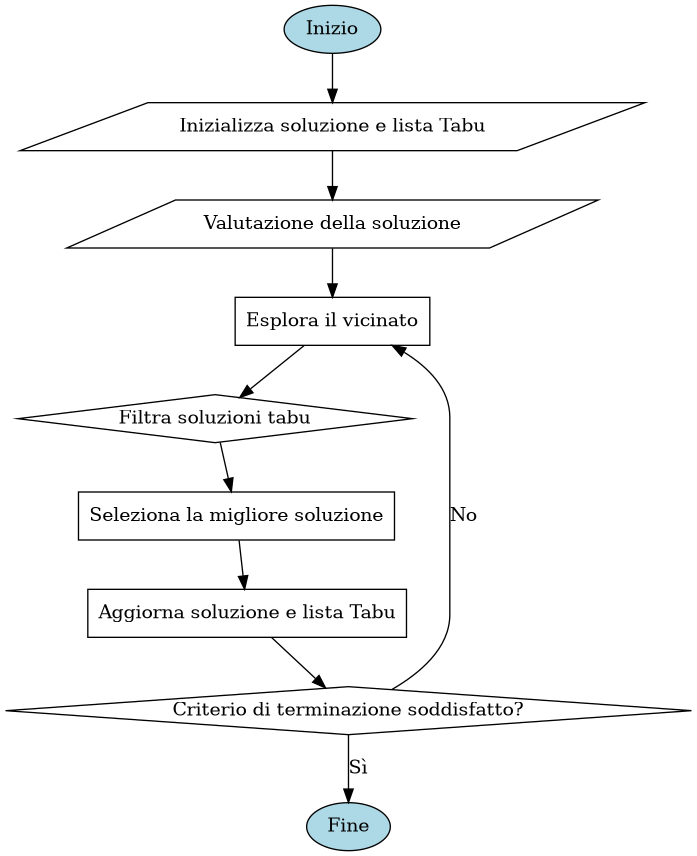
\includegraphics[width=0.50\textwidth]{./img/tabu_search_flowchart.png}
    \caption{Flowchart Tabu Search}
    \label{fig:tabu_search}
\end{figure}

\noindent
Nella terza sezione del progetto si discuterà l'applicazione dell'algoritmo \textit{Tabu Search} al problema enunciato in partenza, il \textit{Weighted Feedback Vertex Set}.

\section{Applicazione dell'algoritmo}\label{s:3}
\subsection{Motivazioni}
Dato il problema presentato nella prima sezione, tra i possibili algoritmi risolutivi, lo studio ha adottato nelle proprie scelte progettuali il \textit{Tabu Search}. Le motivazioni sono varie; il \textit{Tabu Search} è in grado di trovare una soluzione sub-ottimale, avvicinandosi alle migliori soluzioni finora presenti in letteratura per il \textit{WFVS}. Non solo, il tempo di esecuzione dell'algoritmo è promettente, anche nel caso di strutture dati complesse (\textit{i.e Random Graph}). Il \textit{Tabu Search} si adatta facilmente al problema per via della sua natura iterativa che permette di visitare un ampio numero di vicini dei nodi che fanno parte dell'insieme $FVS$. Così facendo rimodella facilmente la propria \textit{Tabu List} e amplifica lo spazio di ricerca all'interno delle strutture dati in esame, avvicinandosi con maggiore successo alla migliore soluzione possibile.


\subsection{Struttura e pseudo-code}
Per procedere nell'analisi del problema, illustriamo il benchmark di istanze utilizzate per testare l'algoritmo implementato e visualizzarne i risultati. Ciascuna istanza nello studio è rappresentata un grafo pesato con una diversa topologia, dimensione $|V|$, densità, e un range di valori per i pesi dei vertici. In particolare, verranno studiati i grafi a griglia (\textit{grid}) e i grafi random. Per i due tipi di grafi sono presenti quindici istanze ciascuno, per un totale di trenta istanze. Lo studio prenderà in esame tre gruppi di cinque istanze per i \textit{Grid Graph}, e tre gruppi di cinque istanze per i \textit{Random Graph}. All'interno di ciascun gruppo, sarà possibile visualizzare la media sulle migliori soluzioni trovate nelle cinque diverse istanze. Inoltre, ciascun esperimento su singola istanza verrà eseguito su 10 \textit{run} indipendenti, ovvero con una soluzione iniziale differente in modo da garantire dei risultati realistici. \\
Nella struttura dell'algoritmo implementato si individuano tre procedure fondamentali per l'espletamento del problema assegnato. In ordine, \verb|generate_initial_|
\verb|solution(G, w)|, \verb|find_fvs_tabu(G, w, maxI, tabuSize, t)|. Di seguito ver\-rà illustrato nel dettaglio il compito di ciascun metodo insieme al proprio pseudo-codice. 
\newline

\begin{algorithm}[H]
\caption{Generazione di una soluzione iniziale per FVS} \label{proc:generate_initial_solution}
\begin{algorithmic}[1]
    \Procedure{GenerateInitialSolution}{G, w}
        \State Ottieni la lista dei nodi dal grafo

        \State Ordina i nodi in base a una funzione di importanza:
        \Statex \hspace{1cm} $\frac{(grado(n))^2}{peso(n)}$ con una componente casuale
        
        \State Inizializza $currentFVS$ come insieme vuoto
        \State Crea una copia temporanea del grafo $tempGraph$

        \For{ogni nodo in $sortedNodes$}
            \State Aggiungi il nodo a $currentFVS$
            \State Rimuovi il nodo da $tempGraph$
            
            \If{$tempGraph$ è una foresta}
                \State \textbf{break} \Comment{Abbiamo trovato una soluzione valida}
            \EndIf
        \EndFor

        \State Inizializza $prunedFVS \gets currentFVS$
        \State Ripristina $tempGraph$ come copia originale del grafo

        \For{ogni nodo in $prunedFVS$, ordinati per peso decrescente e grado crescente}
            \State Rimuovi temporaneamente il nodo da $tempGraph$
            
            \If{$tempGraph$ è ancora una foresta}
                \State Rimuovi definitivamente il nodo da $prunedFVS$
            \Else
                \State Ripristina il nodo e i suoi archi in $tempGraph$
            \EndIf
        \EndFor

        \State \Return $prunedFVS$
    \EndProcedure
\end{algorithmic}
\end{algorithm}

\begin{center}
\textbf{Fig. 1:} Pseudocodice dell’algoritmo di generazione dei candidati iniziali per FVS.
\end{center}

\noindent
Nella Fig.~\ref{proc:generate_initial_solution} viene descritta la strategia per la generazione dei candidati iniziali che soddisfano le condizioni di un insieme $FVS$. Il punto cardine della strategia è l'ordinamento dei nodi: si preferisce dare priorità ai nodi con un alto grado, rafforzando ulteriormente la loro importanza con un elevamento a potenza di due. Si calcola, successivamente, il rapporto con il peso del nodo: più questo è piccolo e maggiore sarà il risultato del rapporto. Questa metrica è stata ideata per lavorare principalmente con nodi critici, che con molta probabilità partecipano ad un ciclo (da qui la considerazione sul grado alto) e il cui peso è minimo, al fine di soddisfare la funzione obiettivo~\eqref{eq:fvs_minimum_weight} definita per questo problema.  \\
Continuando, la procedura effettua una fase di pulizia che ottimizza ulteriormente la scelta dei candidati. La precedente metrica introduce una componente casuale in modo da generare set di candidati diversi ogni volta che la si esegue. Ciò significa che potrebbe introdurre anche nodi con peso alto che non migliorerebbero la funzione obiettivo. L'ordinamento in questa fase, difatti, visualizza per primi i nodi con peso alto e grado molto basso in modo da rimuoverli se possibile.

\begin{algorithm}[H]
\caption{Ricerca di un FVS con Tabu Search} \label{proc:find_fvs_tabu}
\begin{algorithmic}[2]
    \Procedure{FindFvsTabu}{G, w, maxI, tabuSize, t}
        \State Genera una soluzione iniziale $currentFVS$
        \State Inizializza $bestFVS \gets currentFVS$
        \State Calcola il peso minimo iniziale $minWeight$
        \State Inizializza $tabuList$

        \For{$iteration \gets 1$ \textbf{to} $maxI$}
            \State Inizializza $neighbors$ come lista vuota
            \State Ottieni lista dei nodi del grafo
            
            \For{ogni nodo nel grafo}
                \State Genera una nuova soluzione vicina aggiungendo/rimuovendo il nodo
                \State Se la soluzione è in $tabuList$, continua al prossimo nodo
                \State Verifica se la soluzione è valida (il grafo rimanente è una foresta)
                \If{soluzione valida}
                    \State Calcola il peso della nuova soluzione
                    \State Aggiungi la soluzione alla lista dei vicini
                \EndIf
            \EndFor
            
            \If{non ci sono vicini validi} 
                \State \textbf{break} \Comment{Nessuna mossa possibile}
            \EndIf

            \State Seleziona la soluzione con peso minimo tra i vicini
            \State Aggiorna $currentFVS$ e il peso corrente
            
            \If{la nuova soluzione è migliore di $minWeight$}
                \State Aggiorna $bestFVS$ e $minWeight$
                \State Registra l'iterazione come la migliore
                \State Reset contatore iterazioni senza miglioramento
            \Else
                \State Incrementa il contatore iterazioni senza miglioramento
            \EndIf
            
            \If{il numero di iterazioni senza miglioramento $\geq t$}
                \State \textbf{break} \Comment{Early stopping: nessun miglioramento recente}
            \EndIf

            \State Aggiorna la lista Tabu con la nuova soluzione
            \If{dimensione di $tabuList > tabuSize$}
                \State Rimuovi la soluzione più vecchia
            \EndIf
        
        \EndFor

        \State \Return $bestFVS, minWeight$
    \EndProcedure
\end{algorithmic}
\end{algorithm}

\begin{center}
\textbf{Fig. 2:} Pseudocodice della procedura che trova un FVS valido mediante Tabu Search.
\end{center}

\noindent
Nella Fig.~\ref{proc:find_fvs_tabu} viene descritto il metodo del \textit{Tabu Search} applicato al particolare problema. L'algoritmo può effettuare al più 500 iterazioni, tuttavia per una ragionevole convergenza si implementa un meccanismo di \textit{early stopping}: se dopo aver trovato la migliore soluzione si hanno un certo numero di iterazioni (100) senza miglioramenti, l'algoritmo termina. \\
Dopo una serie di esperimenti, la dimensione della \textit{Tabu List} è stata fissata a 15, valore con cui generalmente riesce a fornire dei risultati finali accettabili. \\
Nella sezione successiva e conclusiva, si discuteranno i risultati ottenuti mediante tabelle e grafici. 

\section{Conclusione}\label{s:4}
\subsection{Risultati}
L'algoritmo per lo studio è stato scritto in \textit{Python} ed è stato eseguito su un processore Intel Core Ultra 5 125H.\\
Le tabelle 1. e 2. riportano i risultati ottenuti dall'algoritmo implementato. Nelle tre righe troviamo i tre gruppi formati dalle 5 istanze di un particolare grafo. Nelle colonne, invece, si ha in ordine: la media delle migliori soluzioni trovate per le 5 istanze; la media della deviazione standard delle migliori soluzioni trovate sulle 5 istanze; il numero medio di valutazioni della funzione obiettivo per raggiungere la migliore soluzione su ciascuna delle cinque istanze. Proseguendo, sarà possibile visualizzare i grafici delle curve di convergenza dell'algoritmo su ciascun gruppo e per entrambe le tipologie di grafo.

\begin{table}[H]
\centering
\label{tab:grid_graph}
\begin{tabular}{|c|c|c|c|c|} % 5 colonne centrate con linee verticali
\hline
 & \textbf{Avg. BS} & \textbf{Std. BS} & \textbf{Avg. NV} & \textbf{BS} \\ \hline
\textbf{Grid 5x5} & 216.74 & 21.34 & 1852.66 & 119.8\\ \hline
\textbf{Grid 7x7} & 278.76 & 12.58 & 4220.98 & 252.0\\ \hline
\textbf{Grid 9x9} & 1280.02 & 139.84 & 7051.64 & 1134.4 \\ \hline
\end{tabular}
\caption{Grid Graph} 
\end{table}

\begin{table}[H]
\centering
\label{tab:random_graph}
\begin{tabular}{|c|c|c|c|c|} % 5 colonne centrate con linee verticali
\hline
 & \textbf{Avg. BS} & \textbf{Std. BS} & \textbf{Avg. NV} & \textbf{BS} \\ \hline
\textbf{Rand-100-841} & 1847.32 & 113.68 & 3208.40 & 1724.4\\ \hline
\textbf{Rand-100-3069} & 1150.18 & 20.19 & 994.64 & 1134.0\\ \hline
\textbf{Rand-200-3184} & 5324.98 & 780.64 & 4195.26 & 5135.8 \\ \hline
\end{tabular}
\caption{Random Graph} 
\end{table}

\begin{figure}[H]
\centering
\begin{subfigure}[t]{0.45\textwidth}
\centering
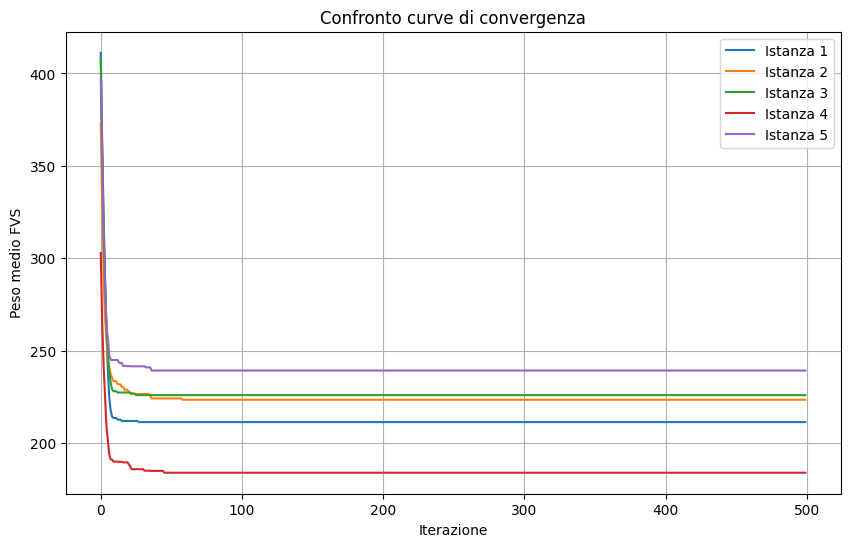
\includegraphics[width=\linewidth]{./img/grid_5_5.png}
\caption{Grid 5x5}
\label{fig:grid1}
\end{subfigure}
\hfill
\begin{subfigure}[t]{0.45\textwidth}
\centering
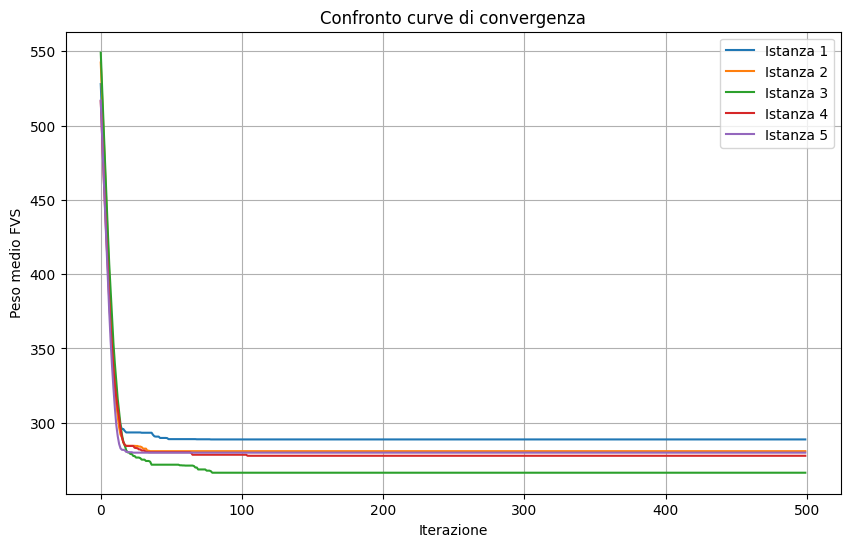
\includegraphics[width=\linewidth]{./img/grid_7_7.png}
\caption{Grid 7x7}
\label{fig:grid2}
\end{subfigure}
\hfill
\begin{subfigure}[t]{0.45\textwidth}
\centering
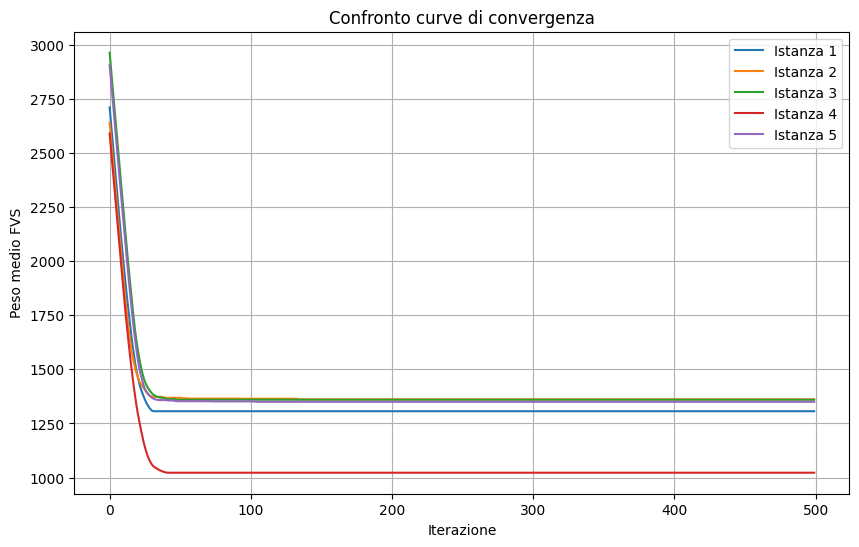
\includegraphics[width=\linewidth]{./img/grid_9_9.png}
\caption{Grid 9x9}
\label{fig:grid3}
\end{subfigure}
\caption{Curve di convergenza per i Grid Graph}
\label{fig:grid_grafici}
\end{figure}

\begin{figure}[H]
\centering
\begin{subfigure}[t]{0.45\textwidth}
\centering
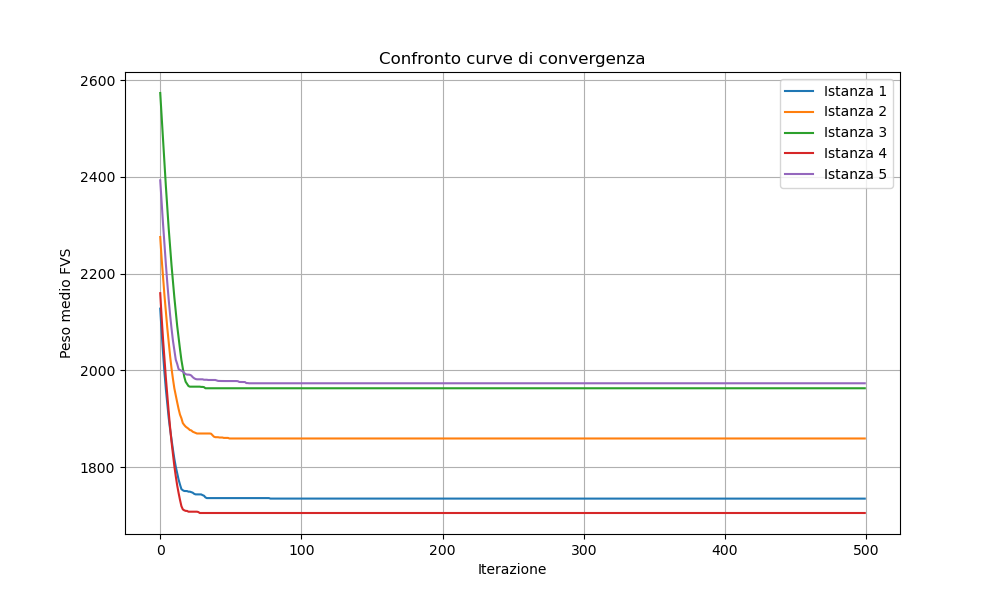
\includegraphics[width=\linewidth]{./img/rand_100_841.png}
\caption{Random 100-841}
\label{fig:rand1}
\end{subfigure}
\hfill
\begin{subfigure}[t]{0.45\textwidth}
\centering
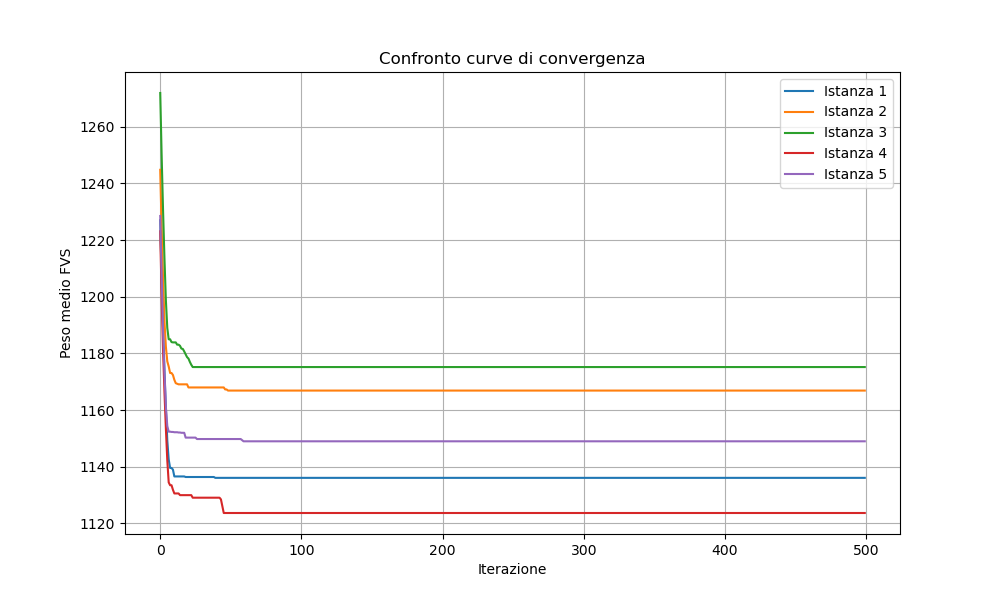
\includegraphics[width=\linewidth]{./img/rand_100_3069.png}
\caption{Random 100-3069}
\label{fig:rand2}
\end{subfigure}
\hfill
\begin{subfigure}[t]{0.45\textwidth}
\centering
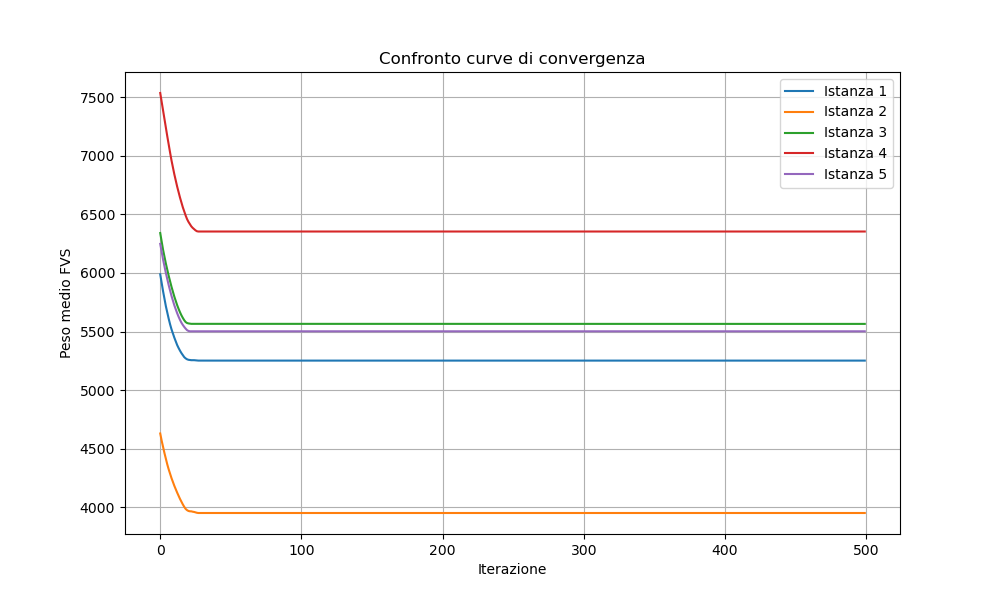
\includegraphics[width=\linewidth]{./img/rand_200_3184.png}
\caption{Random 200-3184}
\label{fig:rand3}
\end{subfigure}
\caption{Curve di convergenza per i Random Graph}
\label{fig:rand_grafici}
\end{figure}

\noindent
Dai risultati visualizzati è possibile notare che l'algoritmo raggiunge la convergenza in poche iterazioni, generalmente meno di un centinaio di esecuzioni risultano sufficienti. Inoltre, nonostante la semplicità dell'algoritmo, la media delle soluzioni trovate sulle cinque istanze di ciascun grafo non si discosta molto dalla rispettiva migliore soluzione presente in letteratura.  

\subsection{Possibili miglioramenti e considerazioni finali}
Nonostante i risultati ottenuti possano sembrare promettenti, è possibile apportare ulteriori migliorie, soprattutto all'interno della logica del \textit{Tabu Search}. L'implemen\-tazione qui discussa è abbastanza semplice e non tiene conto, ad esempio del meccanismo di \textit{Diversification} e \textit{Intensification} che potrebbero espandere ulteriormente lo spazio di ricerca, costruendo un \textit{neighborhood} ancora più adatto al problema. Un'ulteriore strategia potrebbe essere l'implementazione una \textit{Tabu List} dinamica, che varia a seconda della dimensione dell'istanza per adattarsi meglio. Infine, si potrebbe pensare di includere anche l'\textit{Aspiration Criteria} che permette di riammettere le soluzioni \textit{tabu} in opportuni casi.\\
In conclusione, lo studio cerca di avvicinarsi quantopiù a delle soluzioni accettabili per approcciarsi al problema NP-completo del \textit{Weighted Feedback Vertex Set}. Propone un buon compromesso tra il tempo computazionale necessario a trovare una soluzione per questa tipologia di problemi e la qualità del risultato, che può certamente essere migliorata.  


\end{document}
